% main.tex
% Fichero principal de transparencias (incluye a todos los demás).

% Compilar a .pdf con LaTeX (pdflatex)
% Es necesario instalar Beamer (paquete latex-beamer en Debian)
%

% Gráficos:
% Los gráficos pueden suministrarse en PNG, JPG, TIF, PDF, MPS
% Los EPS deben convertirse a PDF (usar epstopdf)
%
%\documentclass[17pt,aspectratio=169,hyperref={pdfusetitle,colorlinks,citecolor=blue,linkcolor=blue,urlcolor=blue}]{beamer}
\documentclass[17pt,aspectratio=169,hyperref={pdfusetitle,colorlinks,allcolors=olive}]{beamer}
\usetheme[orchid]{Hannover}
\beamertemplatenavigationsymbolsempty
\setbeamertemplate{headline}{}
\useoutertheme{infolines}

\usepackage[spanish]{babel}
\usepackage[utf8]{inputenc}
\usepackage{graphics}
%\usepackage{amssymb} % Simbolos matematicos
%\usepackage[pdfusetitle]{hyperref}

\usepackage{chronosys}

%% two slides per page
%\usepackage{pgfpages}
%\pgfpagesuselayout{2 on 1}[a4paper,border shrink=5mm]

\newcommand\YUGE{\fontsize{48}{60}\selectfont}

\newcommand{\secimage}{figs/bookpages}
\AtBeginSection[]
{
  {
    \usebackgroundtemplate{\includegraphics[width=\paperwidth,height=\paperheight]{\secimage}}
    \begin{frame}<beamer>

      \begin{center}
        {\YUGE\bf\insertsection}
      \end{center}
    \end{frame}
  }
  \renewcommand{\secimage}{figs/bookpages}
}


\title[Data mining \& GDPR]{Data mining in the times of the GDPR}
%\subtitle{}
\author[Jesus M. Gonzalez-Barahona]{Jesus M. Gonzalez-Barahona}
\institute[URJC]{Universidad Rey Juan Carlos \\
  @jgbarah ~~~~~ \url{https://jgbarah.github.io/presentations}}

\date{SECO-ASSIST 2019 Research Seminar \\ Uni. Mons (Belgium), September 4th 2019}

\begin{document}

%\begin{frame}[label=firstframe]
\begin{frame}
  \maketitle
\end{frame}



%%%%%%%%%%%%%%%%%%%%%%%%%%%%%%%%%%%%%%%%%%%%%%%%%%%%%%%%%%%%%%%%
%%%%%%%%%%%%%%%%%%%%%%%%%%%%%%%%%%%%%%%%%%%%%%%%%%%%%%%%%%%%%%%%
% lista de temas                                               %
%%%%%%%%%%%%%%%%%%%%%%%%%%%%%%%%%%%%%%%%%%%%%%%%%%%%%%%%%%%%%%%%
%%%%%%%%%%%%%%%%%%%%%%%%%%%%%%%%%%%%%%%%%%%%%%%%%%%%%%%%%%%%%%%%


\definecolor{lightviolet}{HTML}{F4AFF4}
\definecolor{lightorange}{HTML}{FFA17F}
\definecolor{lightgreen}{HTML}{98FB98}
\definecolor{lightred}{HTML}{FF5C5C}
\definecolor{lightblue}{HTML}{89AFCF}
\definecolor{lightbrown}{HTML}{B58868}

%%-----------------------------------------
\begin{frame}[fragile]
  \frametitle{Disclamer}

  \begin{center}
  {\Large
    I'm not a lawyer.\\
    \vspace{.8cm}
    I don't have any \\
    formal training in law.\\
    \vspace{.8cm}
    This is not legal advice.\\
  }
  \end{center}
  
\end{frame}

%%-----------------------------------------
%%-----------------------------------------
\section{Should we worry?}

%%-----------------------------------------
\begin{frame}[fragile]
  \frametitle{Mining software repositories}

  \begin{quote}
    Should we worry \\
    when we research \\
    based on data \\
    extracted from \\
    software development repositories?
  \end{quote}

\end{frame}

%%-----------------------------------------
\begin{frame}[fragile]

  Let's analyze from two (interrelated) \\ points of view: \\

  \vspace{1cm}

  {\large
  \begin{itemize}
  \item legal requirements
  \item ethical requirements
  \end{itemize}
  }
  
\end{frame}

%%-----------------------------------------
\begin{frame}[fragile]
  \begin{center}
    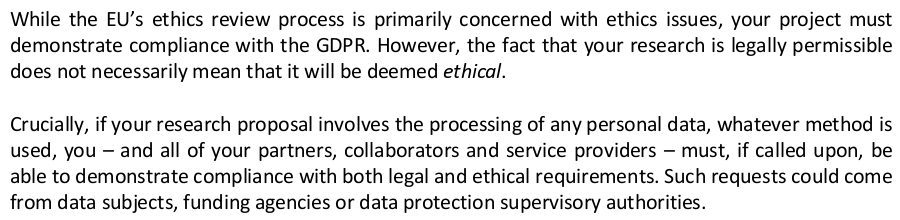
\includegraphics[width=12.5cm]{figs/legal-ethical}
  \end{center}
  {\footnotesize
    \begin{flushright}
    \href{https://ec.europa.eu/research/participants/data/ref/h2020/grants_manual/hi/ethics/h2020_hi_ethics-data-protection_en.pdf}{H2020 document on Ethics and Data Protection},  by EC
    \end{flushright}
  }
\end{frame}

%%-----------------------------------------
\begin{frame}[fragile]
  \frametitle{Applicable law}

  In the European Union (and elsewhere):
  
  \begin{itemize}
  \item \href{https://gdpr.eu/}{General Data Protection Regulation} (GDPR) \\
    Affects all of EU, and rights of EU citizens
  \item Specific law in member states
  \item Recommendations by national data protection agencies \\
  \end{itemize}

  Similar law in other jurisdictions:

  \begin{itemize}
  \item \href{https://www.oag.ca.gov/privacy/ccpa}{California Consumer Privacy Act}
  \end{itemize}
\end{frame}

%%-----------------------------------------
\begin{frame}[fragile]
  \frametitle{Is research exempt?}

  {\Large

    Processing \\
    \vspace{1cm}
    Publication \\
  }
\end{frame}

%%-----------------------------------------
\begin{frame}[fragile]
  \frametitle{Processing}

  Processing of personal data should be:

  \begin{itemize}
  \item lawful,
  \item fair,
  \item and transparent.
  \end{itemize}

  \begin{flushright}
    GDPR, Preface (39)
  \end{flushright}

\end{frame}

%%-----------------------------------------
\begin{frame}[fragile]
  \frametitle{Lawful?}

  \begin{itemize}
  \item explicit consent: difficult when mining repositories
  \item task in the public interest (public institutions)
  \item legitimate interest (non-public institutions)
  \end{itemize}

  \begin{flushright}
    \href{https://www.ukri.org/files/about/policy/ukri-gdpr-faqs-pdf}{GDPR and Research: An Overview for Researchers}, UK Research and Innovation
  \end{flushright}
\end{frame}

%%-----------------------------------------
\begin{frame}[fragile]
  \frametitle{Fair, transparent?}

  Fair, transparent:
  
  \begin{quote}
  Processing for [...] research purposes, shall be subject to appropriate safeguards, in accordance with this Regulation, for the rights and freedoms of
the data subject.
  \end{quote}

  \begin{flushright}
    GDPR, Article 89
  \end{flushright}
\end{frame}

%%-----------------------------------------
\begin{frame}[fragile]
\vspace{-.3cm}
  {\small \em
    Those safeguards shall ensure that technical and organisational measures are in place in particular in order to ensure respect for the principle of data minimisation. Those measures may include pseudonymisation [...]. Where those purposes can be fulfilled by further processing which
does not permit [...] the identification of data subjects, those purposes shall be fulfilled in that manner.
  }

  \begin{flushright}
    GDPR, Article 89
  \end{flushright}
\end{frame}

%%-----------------------------------------
\begin{frame}[fragile]
  \frametitle{Publication}

  Publication of personal data: \\
  \vspace{.2cm}

  {\em
    Sharing personal data should be \\
    through managed processes, \\
    with access and usage controls \\
    to protect from re-identification
  }
  \vspace{.2cm}
  \begin{flushright}
    Potential problem for publication of results, \\
    when they involve personal data (eg: datasets) \\
  \end{flushright}
\end{frame}


%%-----------------------------------------
\begin{frame}[fragile]

  \begin{center}
  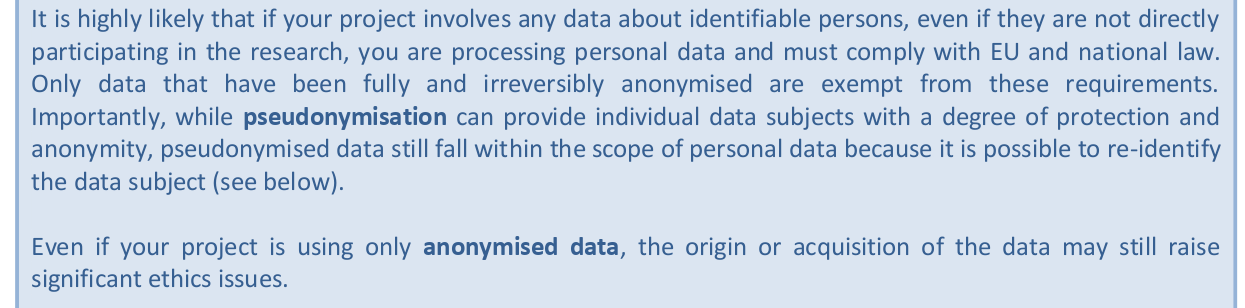
\includegraphics[width=12.5cm]{figs/gdpr-anon-pseudoanon}
  \end{center}
  
  {\footnotesize
    \begin{flushright}
    \href{https://ec.europa.eu/research/participants/data/ref/h2020/grants_manual/hi/ethics/h2020_hi_ethics-data-protection_en.pdf}{H2020 document on Ethics and Data Protection},  by EC
  \end{flushright}
  }
  
\end{frame}

%%-----------------------------------------
\begin{frame}[fragile]

  ``Higher risks'' related to GDPR in research
  
  \begin{center}
  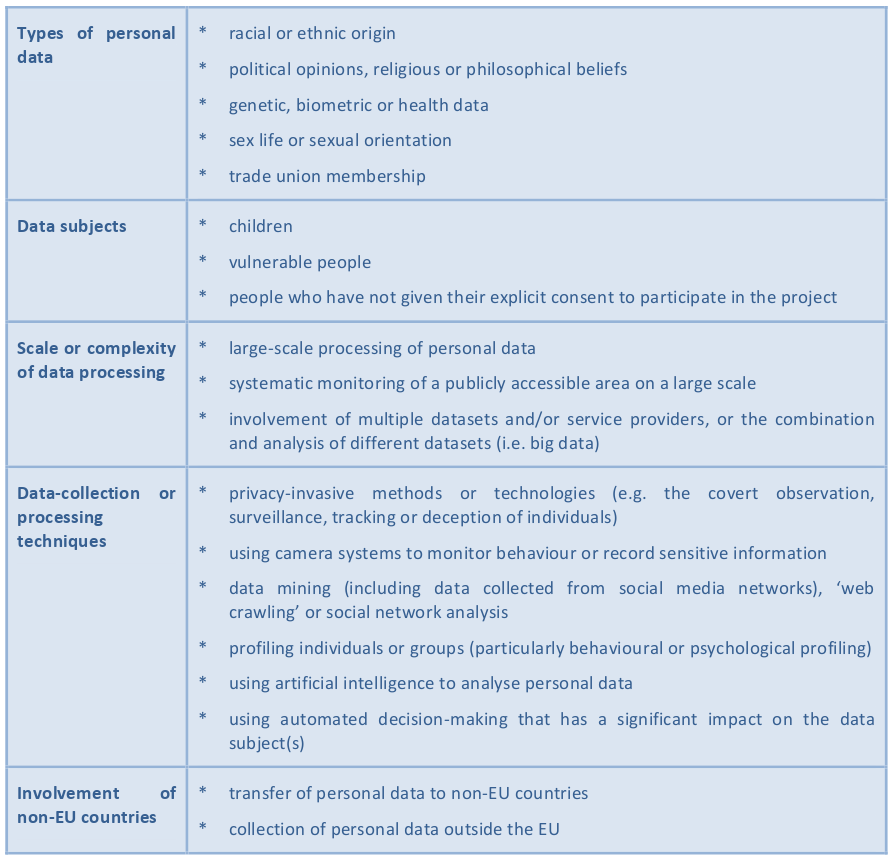
\includegraphics[height=6cm]{figs/gdpr-higher-risks}
  \end{center}
  
  {\footnotesize
    \begin{flushright}
    \href{https://ec.europa.eu/research/participants/data/ref/h2020/grants_manual/hi/ethics/h2020_hi_ethics-data-protection_en.pdf}{H2020 document on Ethics and Data Protection},  by EC
  \end{flushright}
  }
  
\end{frame}

%%-----------------------------------------
\begin{frame}[fragile]
  \vspace{-1.6cm}
  \begin{center}
    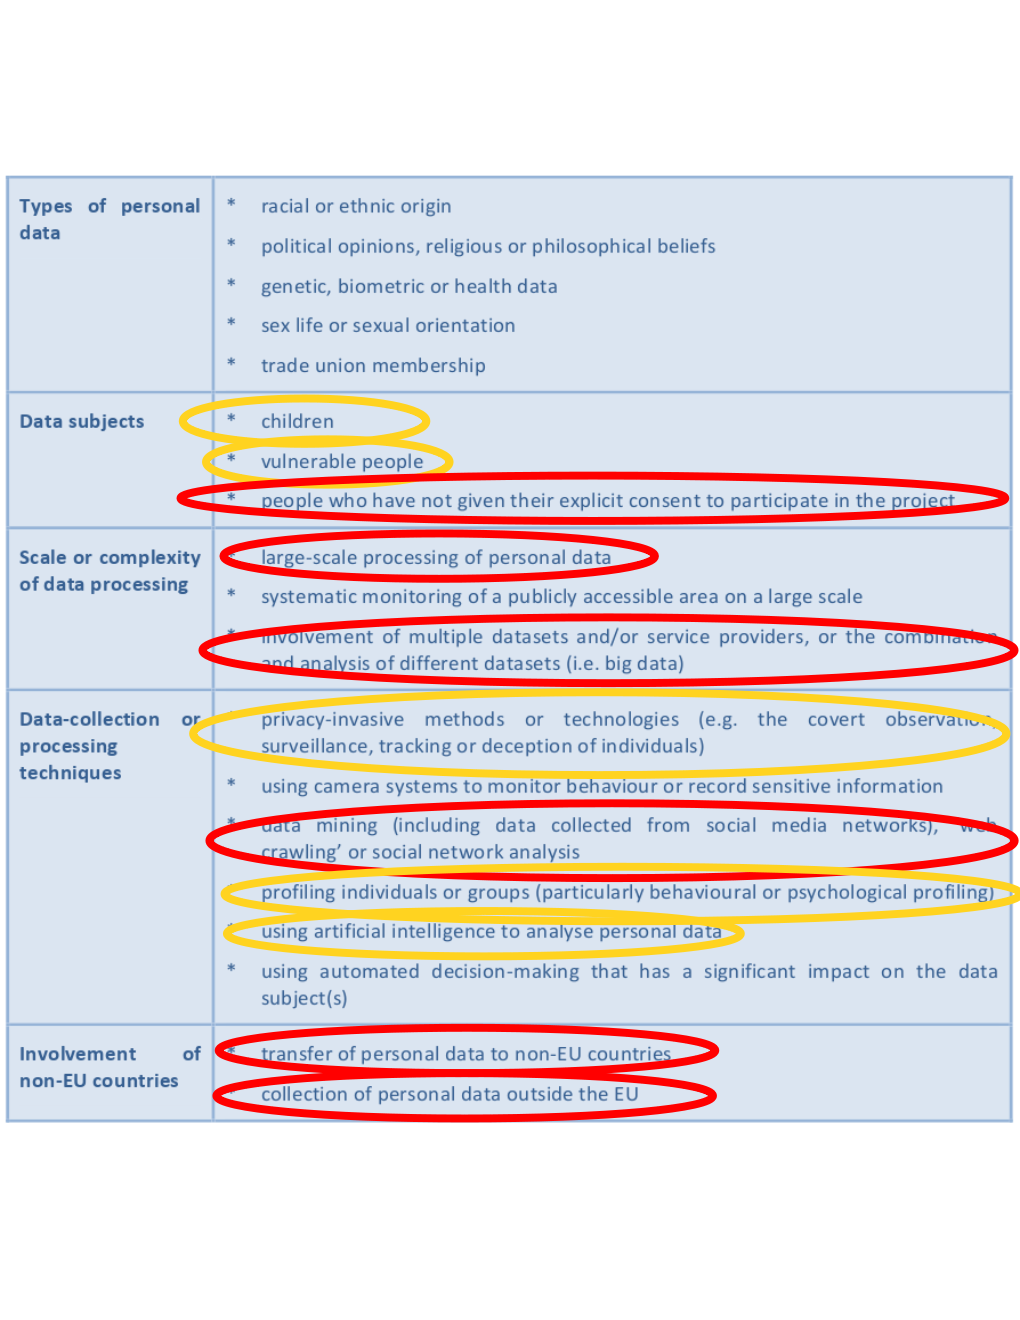
\includegraphics[height=11cm]{figs/gdpr-higher-risks-annotated}
  \end{center}
\end{frame}

%%-----------------------------------------
\begin{frame}[fragile]
  \frametitle{Children \& vulnerable people}

  Maybe we don't know...\\
  ...but they may be in our dataset\\
  
  \begin{itemize}
  \item they are subject to special protection
  \item even when we usually cannot tell who they are...
  \item ...others could
  \end{itemize}

  This situation is very difficult to deal with
\end{frame}

%%-----------------------------------------
\begin{frame}[fragile]
  \frametitle{Privacy invasive methods}

  \begin{itemize}
  \item Example: who is working off-hours

  \item Methodology: tracking individual activity in all available data sources

  \item Risk: tagging specific people
  \end{itemize}
  
  \begin{flushright}
    You can learn working hours, days off, vacation...
  \end{flushright}
\end{frame}

%%-----------------------------------------
\begin{frame}[fragile]
  \frametitle{Profiling individuals or groups}

  \begin{itemize}
  \item Example: activities by newcomers

  \item Methodology: tracking individual activity in all available data sources

  \item Risk: tagging specific people
  \end{itemize}
  
  \begin{flushright}
    You can show specific activity of persons
  \end{flushright}
\end{frame}

%%-----------------------------------------
\begin{frame}[fragile]
  \frametitle{Using AI to analyze personal data}

  \begin{itemize}
  \item Example: find out experts

  \item Methodology: analyze activity to find out experts in some languages, using AI

  \item Risk: singling out specific persons
  \end{itemize}
  
\end{frame}

%%-----------------------------------------
\begin{frame}[fragile]
  \frametitle{Large-scale}

  \begin{itemize}
  \item Usually, several data sources
  \item The more data, the better
  \item If we can combine datasets, we do
  \end{itemize}

  \begin{flushright}
    The better the research, the riskier
  \end{flushright}
\end{frame}

%%-----------------------------------------
\begin{frame}[fragile]
  \frametitle{Data mining from social media}

  \begin{itemize}
  \item Our data source are social media
  \item Of course we mine data from them
  \end{itemize}

  \begin{flushright}
    Data mining is the core of our business
  \end{flushright}
\end{frame}

%%-----------------------------------------
\begin{frame}[fragile]
  \frametitle{No explicit consent}

  \begin{itemize}
  \item We collect data from services...
  \item ...which didn't get explicit consent for our cases
  \item Even if they got, they don't guarantee that for us
  \item In summary: usually, no explicit consent
  \end{itemize}

  \begin{flushright}
    Can we avoid this case?
  \end{flushright}
\end{frame}

%%-----------------------------------------
\begin{frame}[fragile]
  \frametitle{Transfer of data across EU border}

  \begin{itemize}
  \item Collecting data from non EU data sources
  \item Sharing data with non-EU researchers
  \end{itemize}

  \begin{flushright}
    Can we avoid these scenarios?
  \end{flushright}
\end{frame}

%%-----------------------------------------
%%-----------------------------------------
\section{What should we do?}

%%-----------------------------------------
\begin{frame}[fragile]
  \frametitle{Detailed analysis}

  Ethics issues raised by our methodology:

  \begin{itemize}
  \item data collection and processing operations
  \item ethics issues that these raise
  \item mitigation of these issues in practice.
  \end{itemize}

  Submission to the Research Ethics Committee.
\end{frame}

%%-----------------------------------------
\begin{frame}[fragile]
  \frametitle{Detailed analysis}

  \begin{itemize}
  \item Mandatory for EC-funded research proposals

  \item Important: involve the DPO \\
  (Data Protection Officer)

  \item Maybe: requirement to conduct a DPIA \\
    (Data Protection Impact Assessment)
  \end{itemize}
\end{frame}

%%-----------------------------------------
\begin{frame}[fragile]
  \frametitle{GDPR approach}

  Data protection by design (DPbD):\\

  \vspace{.5cm}
  \begin{quote}
    Data  controllers are required  to  implement appropriate technical and organisational measures to give effect to the core data-protection principles of GDPR.
  \end{quote}

  \begin{flushright}
  GDPR, Articles 5 and 25
  \end{flushright}
  
\end{frame}

%%-----------------------------------------
\begin{frame}[fragile]
  \frametitle{DPbD in research}

  Data protection by design:\\

  \begin{itemize}
  \item Anonymization / pseudonymization
  \item data minimization
  \item cryptography (hashing, encrypting)
  \item data protection focused service providers \& storage
  \item procedures for exercising fundamental rights (access, consent)
  \end{itemize}
  
\end{frame}

%%-----------------------------------------
\begin{frame}[fragile]
  \frametitle{Data minimization}

  \begin{quote}
  (1) Data  processing  must  be  lawful,  fair  and  transparent.It  should  involve  only  data  that  are  necessary  and proportionate to achieve the specific task or purpose for which they were collected
  \end{quote}

  \begin{flushright}
    GDPR, Article 5
  \end{flushright}
\end{frame}

%%-----------------------------------------
\begin{frame}[fragile]
  \frametitle{Data minimization}

  \begin{itemize}
  \item Collect minimal personal data
  \item Anonymize and pseudonymize
  \item Store data securely
  \item Dispose data when no longer needed
  \item Limit access to data
  \end{itemize}
\end{frame}

%%-----------------------------------------
\begin{frame}[fragile]
  \frametitle{Mitigation}

  Anonymization, pseudonymization \\
  \vspace{.5cm}
  ...but even in this case, ethics issues: \\

  \begin{itemize}
  \item origin of the data
  \item potential misuse of methodology or findings
  \item potential for deanonymization
  \end{itemize}
\end{frame}

%%-----------------------------------------
%%-----------------------------------------
\section{Some definitions}

%%-----------------------------------------
\begin{frame}[fragile]
  \frametitle{Data processing}

  {\small
    {\em
    (2) Data processing [includes] any operation or set of operations which is performed  on  personal  data  or  on  sets  of  personal  data,  whether  or  not  by  automated  means,  such  as collection,  recording,  organisation,  structuring,  storage,  adaptation  or  alteration,  retrieval,  consultation, use,  disclosure  by  transmission,  dissemination  or  otherwise  making  available,  alignment  or  combination, restriction, erasure or destruction.
    }
  \begin{flushright}
    GDPR, Article 4.
  \end{flushright}
  }
  
\end{frame}

%%-----------------------------------------
\begin{frame}[fragile]
  \frametitle{Actors subject to GDPR}

  \begin{itemize}
  \item Data controller: determines the purposes and means of the processing of personal data
  \item Data processor: processes personal data on behalf of the controller
  \end{itemize}
    
\end{frame}

%%-----------------------------------------
\begin{frame}[fragile]
  \frametitle{Data protection office (DPO)}

  \begin{itemize}
  \item Appointed by controllers and processors \\
    (eg: usually one in each University)
  \item Involved in all issues related to protection of personal data
  \item Data subjects may contact DPO directly
  \item Good, local point to seek advice for a researcher
  \end{itemize}
  
  \begin{flushright}
    GDPR, Articles 37,38,39.
  \end{flushright}
  }
  
\end{frame}

%%-----------------------------------------
\begin{frame}[fragile]
  \frametitle{DPIA}

  Data Protection Impact Assessment:
  \vspace{.3cm}
  
  {\em
    Process designed to   assess   the   data-protection   impacts [...]  and,   [...]  to ensure  that remedial actions are taken as necessary to correct, avoid or minimise the potential negative impacts on the data subjects.
  }
\end{frame}


%%-----------------------------------------
\begin{frame}[fragile]
  \frametitle{DPIA likely required}

\begin{center}
  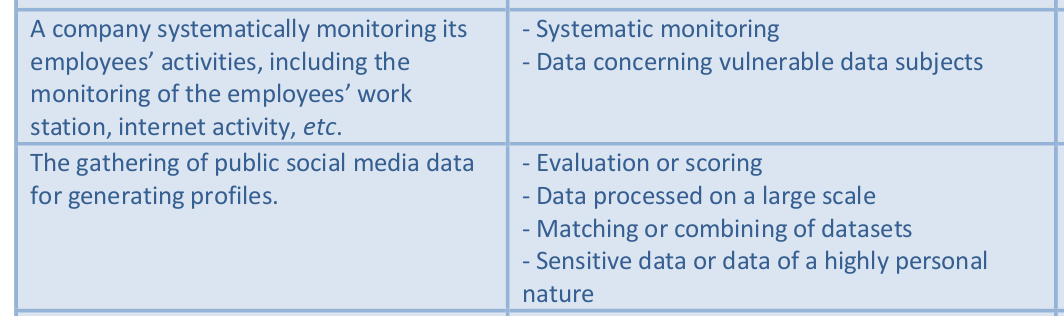
\includegraphics[height=3.9cm]{figs/gdpr-dpia-examples}
  \end{center}  
  
  {\footnotesize
    \begin{flushright}
    \href{https://ec.europa.eu/research/participants/data/ref/h2020/grants_manual/hi/ethics/h2020_hi_ethics-data-protection_en.pdf}{H2020 document on Ethics and Data Protection}, \\ by European Commission
  \end{flushright}
  }
\end{frame}




%%-----------------------------------------
%%-----------------------------------------
\section{A case study}

%%-----------------------------------------
\begin{frame}[fragile]
  \frametitle{The problem}

  You have a collection of \\
  all commits fulfilling some properties \\
  from a large set of public repositories. \\

  \vspace{.3cm}
  
  You analyze number of committers per time period.

  \vspace{.3cm}

  How can you publish the dataset \\
  in a reproduction package? \\
\end{frame}

%%-----------------------------------------
\begin{frame}[fragile]
  \frametitle{The problem}

  \begin{center}
  {\Large
    Let's assume we have \\
    a lawful basis \\
    for the data processing \\
  }
  \end{center}
\end{frame}


%%-----------------------------------------
\begin{frame}[fragile]

{\small
\begin{verbatim}
commit 491f9205c36fdf54b4bbb7f25ba83b6cb99874b9
Author: Jesus M. Gonzalez-Barahona <jgb@gsyc.es>
Date:   Mon May 13 13:33:04 2019 +0200

Add notice about GNOME Extension needed
for indications.
\end{verbatim}  
}

\pause

\begin{center}
  {\Large
    Personal data?
  }
\end{center}

\end{frame}


%%-----------------------------------------
\begin{frame}[fragile]
  \frametitle{Personal data}

  {\footnotesize
  \begin{quotation}
    (1) ‘personal data’ means any information relating to an identified or identifiable natural person (‘data subject’); an identifiable natural person is one who can be identified, directly or indirectly, in particular by reference to an identifier such as a name, an identification number, location data, an online identifier or to one or more factors specific to the physical, physiological, genetic, mental, economic, cultural or social identity of that natural person;
  \end{quotation}
  }
  
  \begin{flushright}
    GDPR, Art. 4
  \end{flushright}
\end{frame}

%%-----------------------------------------
\begin{frame}[fragile]
  \frametitle{Personal data}

  {\footnotesize
    \begin{quotation}
      Personal  data  include  data  such  as  internet  protocol  (IP)  addresses  (unique  identifiers  that  can  be  used  to identify  the  owner  of devices connected to the internet) and data from ‘smart meters’ monitoring energy usage by addresses linked to identifiable persons.
  \end{quotation}
  }

    {\footnotesize
    \begin{flushright}
    \href{https://ec.europa.eu/research/participants/data/ref/h2020/grants_manual/hi/ethics/h2020_hi_ethics-data-protection_en.pdf}{H2020 document on Ethics and Data Protection}, \\ by European Commission
  \end{flushright}
    }

    Certainly, it includes names \& email identifiers.
    
\end{frame}

%%-----------------------------------------
\begin{frame}[fragile]
  \frametitle{Personal data}
  
\begin{verbatim}
Jesus M. Gonzalez-Barahona <jgb@gsyc.es>
\end{verbatim}
  
\end{frame}

%%-----------------------------------------
\begin{frame}[fragile]
  \frametitle{Personal data}

  {\Large
    But... wait!!!! \\
    \vspace{1cm}
    Our data is public data!! \\
  }
\end{frame}

%%-----------------------------------------
\begin{frame}[fragile]
  \frametitle{Open source data}

  \begin{center}
  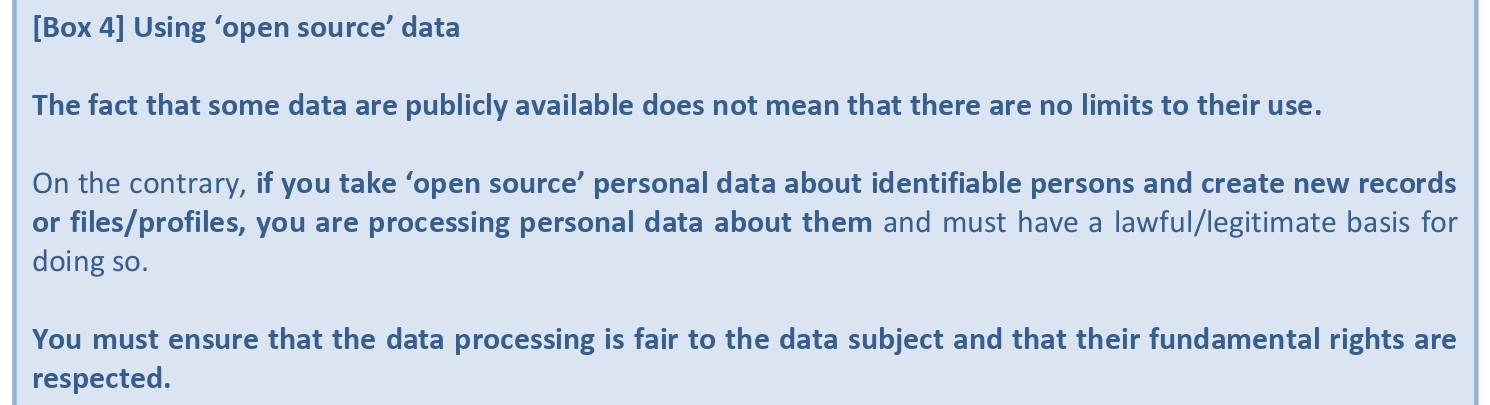
\includegraphics[width=12cm]{figs/gdpr-open-source-data}
  \end{center}  
  
  {\footnotesize
    \begin{flushright}
    \href{https://ec.europa.eu/research/participants/data/ref/h2020/grants_manual/hi/ethics/h2020_hi_ethics-data-protection_en.pdf}{H2020 document on Ethics and Data Protection}, \\ by European Commission
  \end{flushright}
  }
\end{frame}

%%-----------------------------------------
\begin{frame}[fragile]
  \frametitle{Open source data}

  \begin{center}
  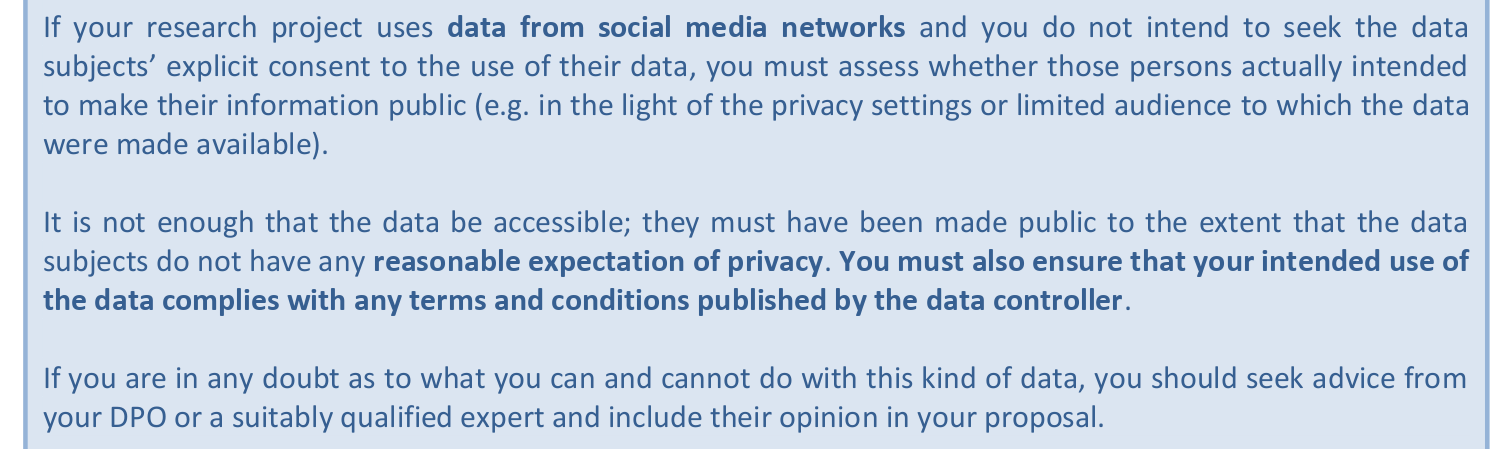
\includegraphics[width=12cm]{figs/gdpr-open-source-data-b}
  \end{center}  

  {\footnotesize
    \begin{flushright}
    \href{https://ec.europa.eu/research/participants/data/ref/h2020/grants_manual/hi/ethics/h2020_hi_ethics-data-protection_en.pdf}{H2020 document on Ethics and Data Protection}, \\ by European Commission
  \end{flushright}
  }
\end{frame}

%%-----------------------------------------
\begin{frame}[fragile]
  \frametitle{How to fix the problem}
  
  \begin{itemize}
  \item Anonymize: Strip all personal data \\
    (but still... more on this later)
  \item Pseudonymize personal data \\
    (the dataset will be much richer, but still...)
  \end{itemize}
\end{frame}

%%-----------------------------------------
\begin{frame}[fragile]
  \frametitle{Pseudonymizing}

  {\footnotesize
  \begin{quotation}
    (5) ‘pseudonymisation’ means the processing of personal data in such a manner that the personal data can no longer be attributed to a specific data subject without the use of additional information, provided that such additional information is kept separately and is subject to technical and organisational measures to ensure that the personal data are not attributed to an identified or identifiable natural person;
  \end{quotation}
  }
  
  \begin{flushright}
    GDPR, Art. 4
  \end{flushright}
\end{frame}

%%-----------------------------------------
\begin{frame}[fragile]
  \frametitle{Pseudonymization}

  \begin{center}
  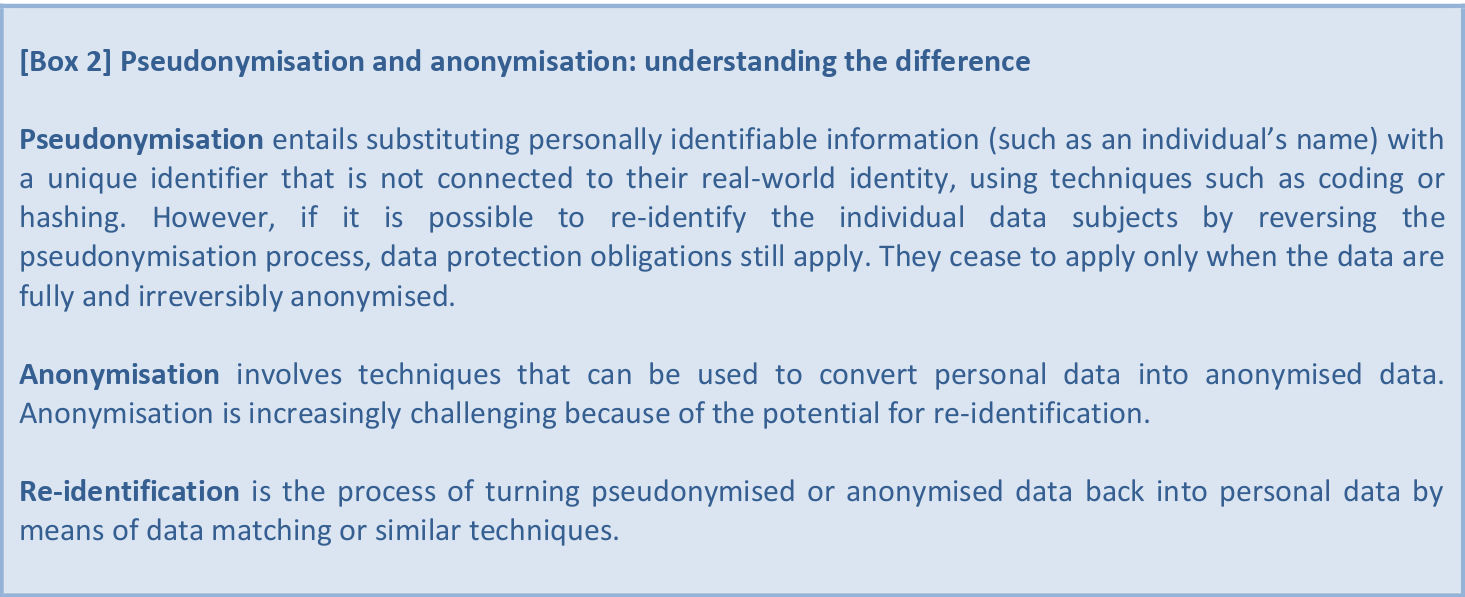
\includegraphics[width=11cm]{figs/gdpr-pseudonymization}
  \end{center}  
  
  {\footnotesize
    \begin{flushright}
    \href{https://ec.europa.eu/research/participants/data/ref/h2020/grants_manual/hi/ethics/h2020_hi_ethics-data-protection_en.pdf}{H2020 document on Ethics and Data Protection}, \\ by EC
  \end{flushright}
  }
\end{frame}

%%-----------------------------------------
\begin{frame}[fragile]
  \frametitle{Pseudonymizing 1}

{\small
\begin{verbatim}
echo -n "<jgb@gsyc.es>" | sha256sum 
3fdffb4a435cc3a5bab7d96b3cc2cefea90ca879f7fba034716c42d374f0cb81 -
\end{verbatim}
}  

{\small
\begin{verbatim}
commit 491f9205c36fdf54b4bbb7f25ba83b6cb99874b9
Author: 3fdffb4a435cc3a5bab7d96b3cc2cefea90ca879f7fba034716c42d374f0cb81
Date:   Mon May 13 13:33:04 2019 +0200

Add notice about GNOME Extension needed...
\end{verbatim}  
}

\end{frame}

%%-----------------------------------------
\begin{frame}[fragile]
  \frametitle{Pseudonymizing 1}

Not good enough:

  \begin{center}
  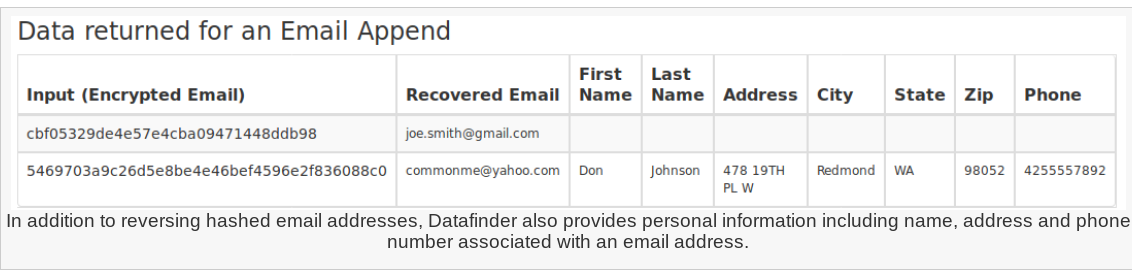
\includegraphics[width=12cm]{figs/email-hash}
  \end{center}  

  \begin{flushright}
  {\small
\href{https://freedom-to-tinker.com/2018/04/09/four-cents-to-deanonymize-companies-reverse-hashed-email-addresses/}{Four cents to deanonymize: Companies reverse hashed email addresses}, by Gunes Acar
  }
  \end{flushright}  
\end{frame}

%%-----------------------------------------
\begin{frame}[fragile]
  \frametitle{Pseudonymizing 1}

For the curious:

\begin{itemize}
\item Estimated: 5 billion email addresses (2018)
\item Amazon EC2: 450 billion hashes/sec.
\item Lists of (targeted) email lists for sale
\item Data breaches leaking billions of addresses
\end{itemize}

There is a whole business ecosystems around email addresses

  \begin{flushright}
  {\small
\href{https://freedom-to-tinker.com/2018/04/09/four-cents-to-deanonymize-companies-reverse-hashed-email-addresses/}{Four cents to deanonymize: Companies reverse hashed email addresses}, by Gunes Acar
  }
  \end{flushright}  

\end{frame}

%%-----------------------------------------
\begin{frame}[fragile]
  \frametitle{Pseudonymizing 2}

  \begin{itemize}
  \item Hash ``name + address'' \\
  \end{itemize}

  Better, but still subject to attack if you harvested addresses

  \begin{itemize}
  \item Salt the hash, use different algorithm \\
  \item Non-hash functions (eg, sequential code)
  \item Encryption instead of hash
  \end{itemize}

  Better, but you need to disclose details \\
  if you want others to merge with your dataset

\end{frame}

%%-----------------------------------------
\begin{frame}[fragile]
  \frametitle{Pseudonymizing 3}

  A possibility emerges:

  \begin{quotation}
    ``Encryption / coding \\
    \vspace{.3cm}
    Datasets: public \\
    Key / coding table: \\
    only to researchers asking for it \\
  \end{quotation}

    (variant: reference them in the paper) \\
    \vspace{.3cm}

  Is this good enough for ``legitimate use''? \\
\end{frame}

%%-----------------------------------------
\begin{frame}[fragile]
  \frametitle{Pseudonymizing 3}

{\small
\begin{verbatim}
commit 491f9205c36fdf54b4bbb7f25ba83b6cb99874b9
Author: 4334345
Date:   Mon May 13 13:33:04 2019 +0200

Add notice about GNOME Extension needed...
\end{verbatim}  
}

Separate table:

{\small
\begin{verbatim}
4334345,Jesus M. Gonzalez-Barahona <jgb@gsyc.es>
\end{verbatim}  
}

\end{frame}

%%-----------------------------------------
\begin{frame}[fragile]
  \frametitle{We still have a problem}

  \begin{center}
  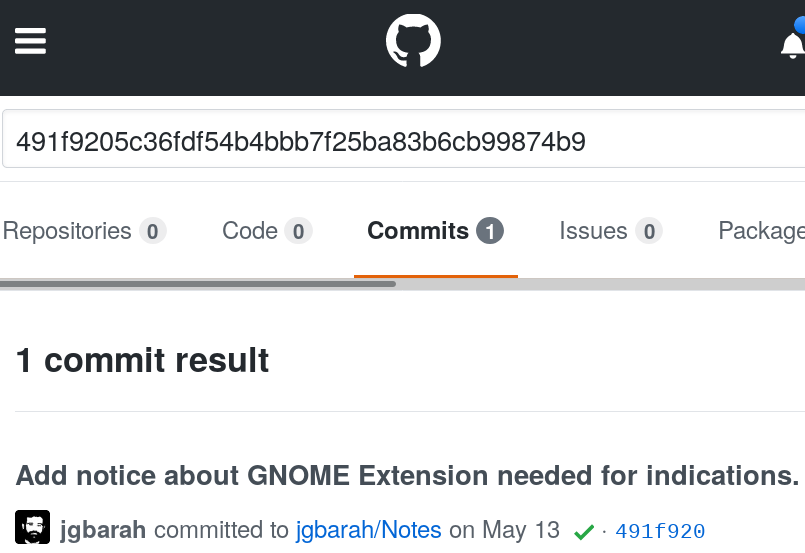
\includegraphics[width=8cm]{figs/github-hash}
  \end{center}  
  
\end{frame}

%%-----------------------------------------
\begin{frame}[fragile]
  \frametitle{We still have a problem}

{\small
\begin{verbatim}
curl https://archive.softwareheritage.org/api/1/revision/
  491f9205c36fdf54b4bbb7f25ba83b6cb99874b9/

{"author":
  {"name":"Jesus M. Gonzalez-Barahona",
   "fullname":"Jesus M. Gonzalez-Barahona <jgb@gsyc.es>",
   "email":"jgb@gsyc.es"}
  }
  ...
}
\end{verbatim}  
}

\end{frame}

%%-----------------------------------------
\begin{frame}[fragile]
  \frametitle{What can we do?}

  Pseudonymize the hash too:

{\small
\begin{verbatim}
commit 6777888876876
Author: 4334345
Date:   Mon May 13 13:33:04 2019 +0200

Add notice about GNOME Extension needed...
\end{verbatim}  
}
  
\end{frame}

%%-----------------------------------------
\begin{frame}[fragile]
  \frametitle{We still have a problem (2)}

  \begin{center}
  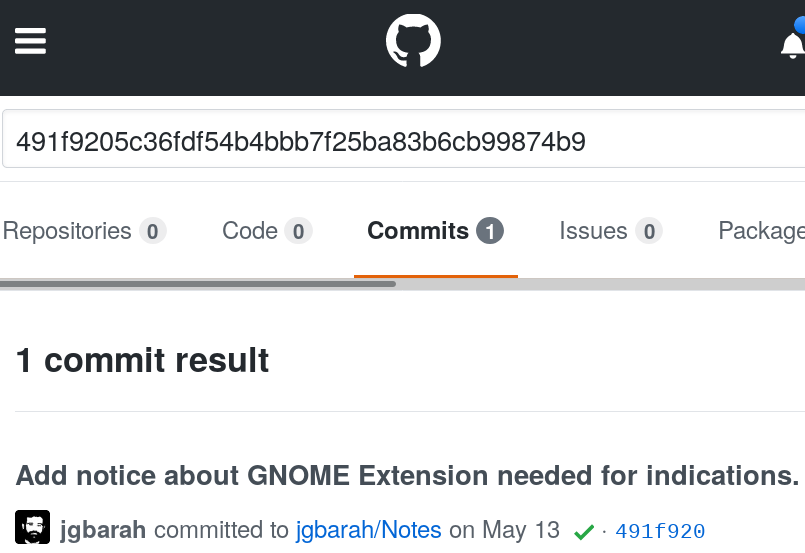
\includegraphics[width=8cm]{figs/github-hash}
  \end{center}  
  
\end{frame}

%%-----------------------------------------
\begin{frame}[fragile]
  \frametitle{We still have a problem (2)}

  \begin{itemize}
  \item Commit comment can be used to deanonymize author.
  \item Date can be used to deanonymize author.
  \end{itemize}

{\small
\begin{verbatim}
commit 6777888876876
Author: 4334345
Date:   5353453453
Comment: 4343434334
\end{verbatim}  
}

...and separate coding tables
\end{frame}

%%-----------------------------------------
\begin{frame}[fragile]
  \frametitle{Why we need tables}

  \begin{itemize}
  \item For reproduction: commits per time period
  \item for reuse: identity merging
  \item for reuse: relationship between message and time of the day
  \item for reuse: link to issues
  \item ...
  \end{itemize}
  
\end{frame}

%%-----------------------------------------
\begin{frame}[fragile]
  \frametitle{When data is public...}

  This is a problem for anyone \\
  having access to the data \\
  that allows deanonymization \\

  \vspace{.5cm}
  
  But also for anyone letting others deanonymize \\

  \vspace{.5cm}
  
  Big trouble if it is publicly available data \\
  
\end{frame}


%%-----------------------------------------
%%-----------------------------------------
\section{Important details}

%%-----------------------------------------
\begin{frame}[fragile]
  \frametitle{Timing of anonymization}

  \begin{itemize}
  \item Collection (no personal data is processed) \\
    Example: web form, no browser tracking \\
    Example: anonymous dataset from 3rd party \\
  \item Later than collection: \\
    Raw data is not anonymized \\
    (needs special protection) \\
  \end{itemize}
  
\end{frame}

%%-----------------------------------------
\begin{frame}[fragile]
  \frametitle{Informed consent}

  \begin{quote}
  Explain to participants what your research is about, what their participation in your project will entail and any risks that may be involved. When they have fully understood, see and obtain their express permission.
  \end{quote}

  \begin{flushright}
  GDPR, Article 4 (11), Article 7
  \end{flushright}
\end{frame}

%%-----------------------------------------
\begin{frame}[fragile]
  \frametitle{Managing consent}

  You need to document and archive consent

  You need to be able of producing evidence

  Consent management applications:

  \begin{itemize}
  \item ethically robust, secure
  \item model consent processes
  \item manage, document, evidence
  \end{itemize}
\end{frame}

%%-----------------------------------------
\begin{frame}[fragile]
  \frametitle{Secondary use}

  Usually, we perform secondary use \\
  (we don't collect data directly from persons) \\

  \vspace{.5cm}

  Important: check original consent \\

  \vspace{.5cm}

  Explain how data was obtained, \\
  justify use (legitimate use) \\
  ensure processing is fair to data subjects \\
\end{frame}

%%-----------------------------------------
\begin{frame}[fragile]
  \frametitle{Secondary use}


  {\em
    (47) the legitimate interests of a controller [...] or of a third party, may provide a legal basis for processing, provided that  the  interests  or  the  fundamental  rights  and  freedoms  of  the  data  subject  are  not  overriding,  taking into  consideration  the  reasonable  expectations  of  data  subjects  based  on  their  relationship  with  the controller
  }

  \begin{flushright}
    GDPR, Preamble (see also Art. 89)
  \end{flushright}
\end{frame}

%%-----------------------------------------
\begin{frame}[fragile]
  \frametitle{Data security}

 
  \begin{itemize}
  \item Appropriate  technical \& organisational measures
  \item Level of security commensurate to risks faced by the  data  subjects
  \item Prevention of unauthorized access, disclosure, accidental deletion
  \end{itemize}
\end{frame}

%%-----------------------------------------
\begin{frame}[fragile]
  \frametitle{Data security}

  \begin{center}
  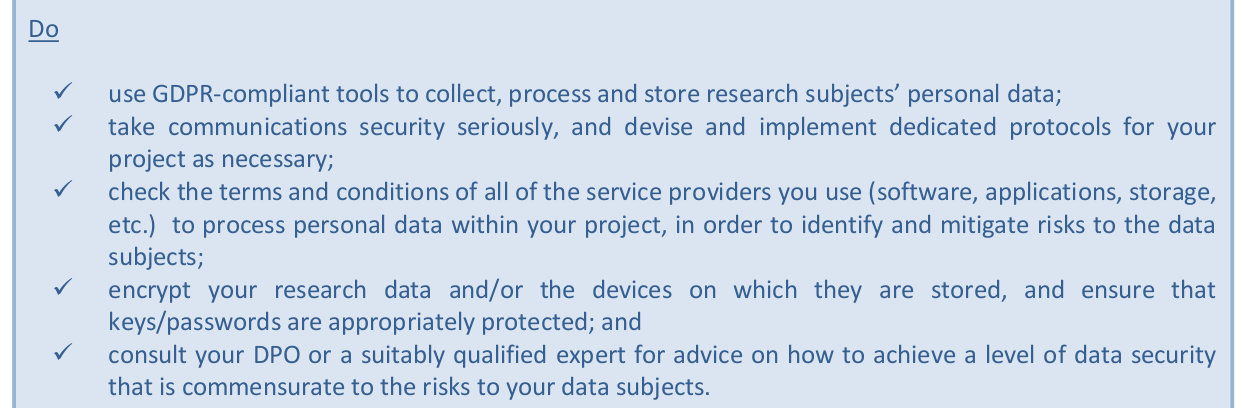
\includegraphics[width=12cm]{figs/gdpr-data-security}
  \end{center}  
  
  {\footnotesize
    \begin{flushright}
    \href{https://ec.europa.eu/research/participants/data/ref/h2020/grants_manual/hi/ethics/h2020_hi_ethics-data-protection_en.pdf}{H2020 document on Ethics and Data Protection}, \\ by EC
  \end{flushright}
  }
 
\end{frame}

%%-----------------------------------------
\begin{frame}[fragile]
  \frametitle{Data security}

  \begin{center}
  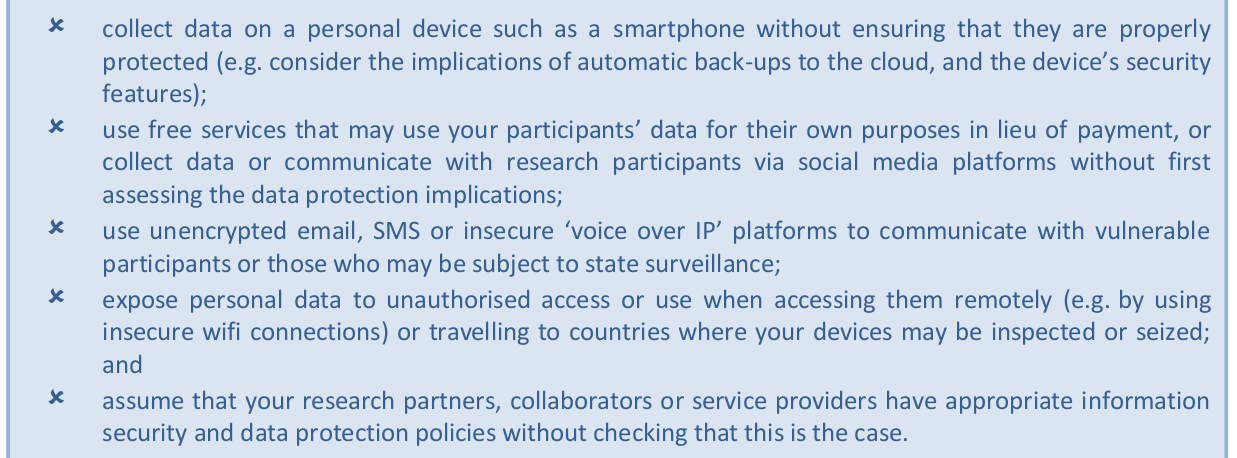
\includegraphics[width=12cm]{figs/gdpr-data-security-b}
  \end{center}  
  
  {\footnotesize
    \begin{flushright}
    \href{https://ec.europa.eu/research/participants/data/ref/h2020/grants_manual/hi/ethics/h2020_hi_ethics-data-protection_en.pdf}{H2020 document on Ethics and Data Protection}, \\ by EC
  \end{flushright}
  }
 
\end{frame}

%%-----------------------------------------
\begin{frame}[fragile]
  \frametitle{Transfer outside EU}

  Possible (GPDR, Chapter 5)::

  \begin{itemize}
  \item to countries with ``adequacy  determination''
  \item when explicit consent is obtained
  \item when compliant data-transfer agreements are in place
  \end{itemize}

  Beware of third-party services!!!
  
  \begin{flushright}
    \href{https://ec.europa.eu/info/law/law-topic/data-protection/international-dimension-data-protection/adequacy-decisions_en}{Non-EU countries with adequacy determination}
  \end{flushright}
 
\end{frame}

%%-----------------------------------------
\begin{frame}[fragile]
  \frametitle{Transfer outside EU}

  \begin{center}
  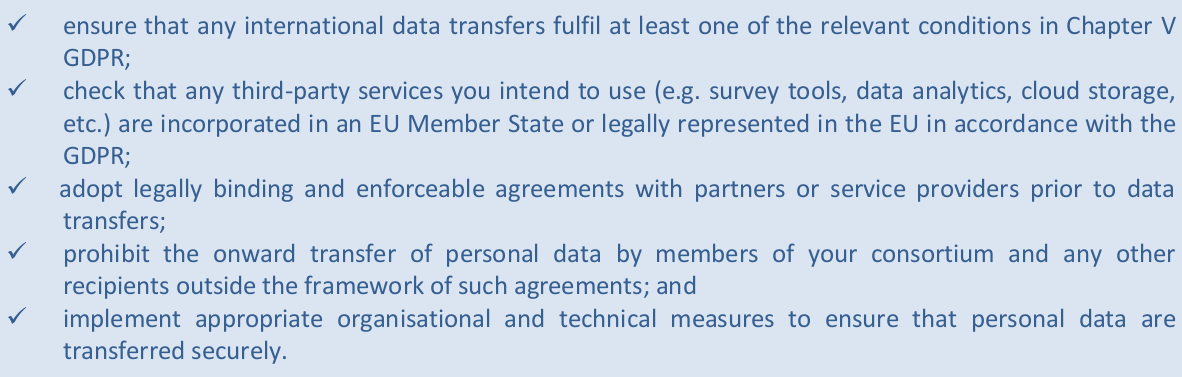
\includegraphics[width=12cm]{figs/gdpr-intl-transfers}
  \end{center}  
  
  {\footnotesize
    \begin{flushright}
    \href{https://ec.europa.eu/research/participants/data/ref/h2020/grants_manual/hi/ethics/h2020_hi_ethics-data-protection_en.pdf}{H2020 document on Ethics and Data Protection}, \\ by EC
  \end{flushright}
  }
 
\end{frame}

%%-----------------------------------------
\begin{frame}[fragile]
  \frametitle{Archiving}

  Archive personal data \\
  only as needed for research purposes. \\
  \vspace{.3cm}
  Delete it as soon as possible \\
  (define a maximum retention period). \\
  \vspace{.3cm}
  Beware of backups and data in cloud storage.
  
  {\footnotesize
    \begin{flushright}
    \href{https://ec.europa.eu/research/participants/data/ref/h2020/grants_manual/hi/ethics/h2020_hi_ethics-data-protection_en.pdf}{H2020 document on Ethics and Data Protection}, \\ by EC
  \end{flushright}
  }
\end{frame}

%%-----------------------------------------
\begin{frame}[fragile]
  \frametitle{Archiving}

But you can keep personal data indefinitely if you ensure it is only for:

\begin{itemize}
\item archiving purposes in the public interest
\item scientific or historical research purposes
\item statistical purposes
\end{itemize}

\end{frame}

%%-----------------------------------------
\begin{frame}[fragile]
  \frametitle{Archiving}

  \begin{center}
    {\Large
      Open issue: \\
      archiving for reproduction \\
    }
  \end{center}

  \vspace{.5cm}
  In principle, covered by research exemption, \\
    but it is not absolute\\
    
\end{frame}

%%-----------------------------------------
\begin{frame}[fragile]
  \frametitle{Collection outside EU}

  Subject to GDPR \\
  even if data comes from outside EU \\
  if data controller is based in EU \\

  \vspace{1cm}
  
  Of course, compliance with \\
  the law of the country of collection \\
\end{frame}


%%-----------------------------------------
\begin{frame}[fragile]
\frametitle{Children}

{\small
    \begin{quote}
  If your research project involves collecting data from children, you must follow the ``EC Guidance note on informed consent'', in  particular the provisions on obtaining  the  consent  of  a  parent/legal representative  and,  where  appropriate,  the  assent  of  the  child.
    \end{quote}

  \begin{flushright}
    \href{https://ec.europa.eu/research/participants/data/ref/h2020/grants_manual/hi/ethics/h2020_hi_ethics-data-protection_en.pdf}{H2020 document on Ethics and Data Protection}, European Commission
  \end{flushright}

  }
  
\end{frame}

%%-----------------------------------------
\begin{frame}[fragile]

  {\small
    \begin{quote}
The  GDPR establishes special safeguards for children in relation to ``information  society  services'',  a broad term covering all internet service providers, including social media platforms. These include a requirement for verified parental consent in respect of information society services offered directly to  children aged under 16. Individual Member States may  provide for this threshold to  be lowered to 13.
    \end{quote}

  \begin{flushright}
    \href{https://ec.europa.eu/research/participants/data/ref/h2020/grants_manual/hi/ethics/h2020_hi_ethics-data-protection_en.pdf}{H2020 document on Ethics and Data Protection}, European Commission
  \end{flushright}

  }
  
\end{frame}

%%-----------------------------------------
%%-----------------------------------------
\section{Call for action}

%%-----------------------------------------
\begin{frame}[fragile]
  \frametitle{Researchers \& developers}

  Maybe we researchers need to work \\
  with developers \\
  to learn what is legitimate use for them? \\
  \vspace{.5cm}
  
  Maybe developers should specify \\
  what is legitimate use for them, \\
  in their repositories? \\
  
\end{frame}

%%-----------------------------------------
\begin{frame}[fragile]
  \frametitle{An inspiration}
  
  \begin{columns}[T]
    \begin{column}{.58\textwidth}
      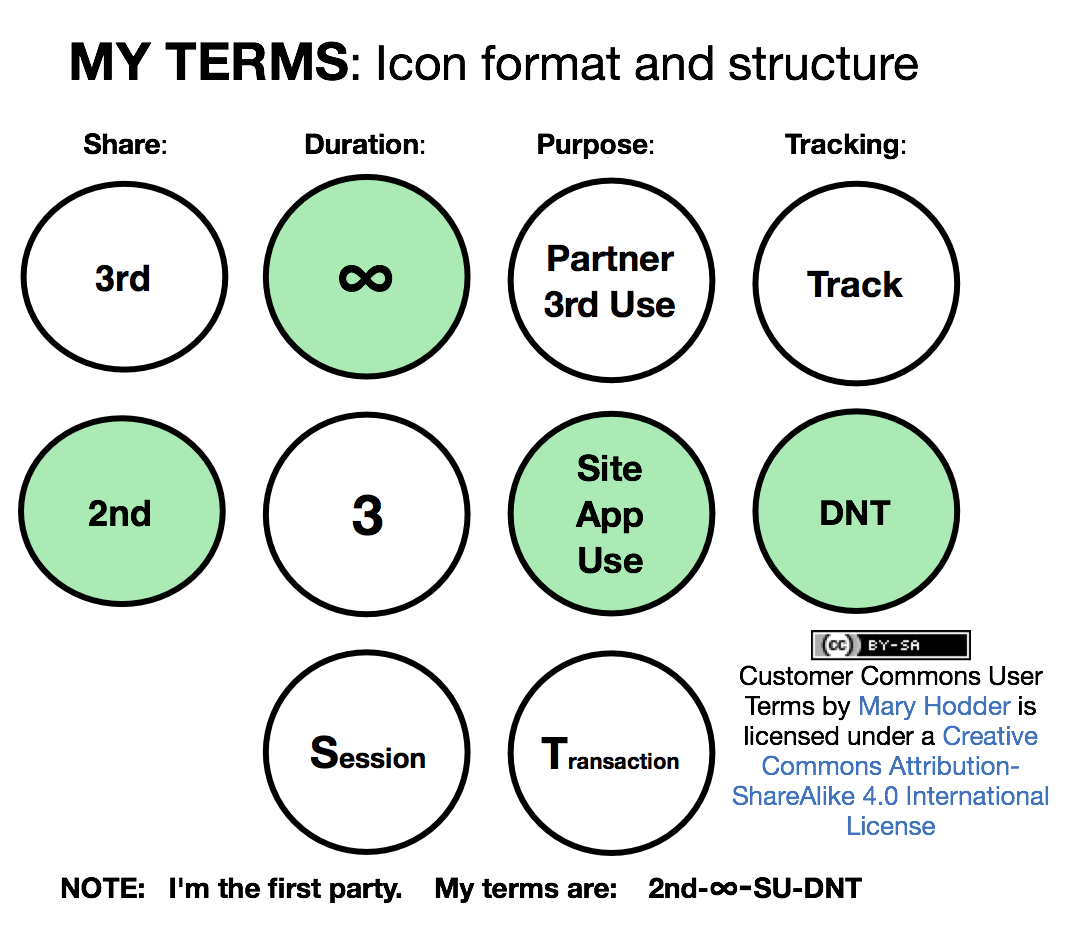
\includegraphics[height=6cm]{figs/user-terms}
    \end{column}%
    \hfill%
    \begin{column}{.40\textwidth}
      {\footnotesize
        ~
        \vspace{3cm}
        \begin{flushright}
          \href{https://kantarainitiative.org/confluence/display/infosharing/User+Submitted+Terms+--+UX+and+Interface+V.1}{User Submitted Terms}, by Mary Hooder \\
          \href{http://customercommons.org/2014/10/27/customer-commons-and-user-submitted-terms/}{Customer Commons and User Submitted Terms} \\
        \end{flushright}
      }
    \end{column}%
  \end{columns}

\end{frame}

%%-----------------------------------------
\begin{frame}[fragile]
  \frametitle{A related IEEE WG}

  \begin{center}
    
\includegraphics[width=12cm]{figs/ieee-wg}
  \end{center}

  \begin{flushright}
    \href{https://standards.ieee.org/project/7012.html}{Machine Readable Privacy Terms Working Group}
  \end{flushright}
\end{frame}

%%-----------------------------------------
\begin{frame}[fragile]
  \frametitle{FOSS is open for a reason}

  Having the source code available \\
  is a conscious decision\\
  \vspace{.3cm}
  It could be extended to all data \\
  related to software development \\
  (better understanding of the project) \\
  \vspace{.3cm}
  Clarification of intent would help to define legitimate interest and prove ethics compliance
\end{frame}



%%-----------------------------------------
%%-----------------------------------------
\section{To probe further}


%%-----------------------------------------
\begin{frame}[fragile]
  \frametitle{References}

  \begin{itemize}
  \item \href{https://gdpr.eu/}{GDPR portal} by EC \\
    (includes full text of GDPR)
  \item \href{https://ec.europa.eu/research/participants/data/ref/h2020/grants_manual/hi/ethics/h2020_hi_ethics-data-protection_en.pdf}{H2020 document on Ethics and Data Protection}, European Commission
  \item \href{https://www.ukri.org/files/about/policy/ukri-gdpr-faqs-pdf}{GDPR and Research: An Overview for Researchers}, UK Research and Innovation
  \end{itemize}
  
\end{frame}


%%-----------------------------------------
\begin{frame}[fragile]
  \frametitle{Credits}

  
\end{frame}



\frame{
~
\vspace{1cm}

\begin{flushright}


\includegraphics[width=2.2cm]{figs/by-sa}
 \\

\begin{footnotesize}
\copyright 2019 Jesus M. Gonzalez-Barahona. \\

\vspace{.4cm}

Some rights reserved. This document is distributed under the terms of the Creative Commons License ``Attribution-ShareAlike 4.0'',
available in \\
{\scriptsize \url{http://creativecommons.org/licenses/by-sa/4.0/}} \\

\vspace{.4cm}

This document (including source) is available from
\url{https://jgbarah.github.io/presentations}

\end{footnotesize}
\end{flushright}

}
%%

%\againframe{firstframe}

\end{document}
